\documentclass[11pt]{article}
\usepackage[a4paper, margin=2cm]{geometry}
\usepackage{graphicx}
\usepackage{hyperref}
\usepackage{enumitem}
\usepackage{subcaption}
\usepackage{amsmath}
\usepackage{float}
% !TeX spellcheck = en_GB 

\title{Report: Bayesian Networks DAG Testing}
\date{11 November 2018}
\author{Niek Janssen (s??)\and Laurens Kuiper (s4467299)\and Ward Theunisse (s4492765)}

\begin{document}
\maketitle
\thispagestyle{empty}
\newpage
\section{Introduction}
In this report we present the findings of testing and amending the initial model as proposed in our exposee.
The model was iteratively tested using the $\chi^2$-test, removing and adding variables/connections at each step.

\section{Initial DAG}
Our initial DAG as shown in \autoref{fig:initial_dag} was constructed with our prior beliefs about the data.

\begin{figure}[h]
	\centering
	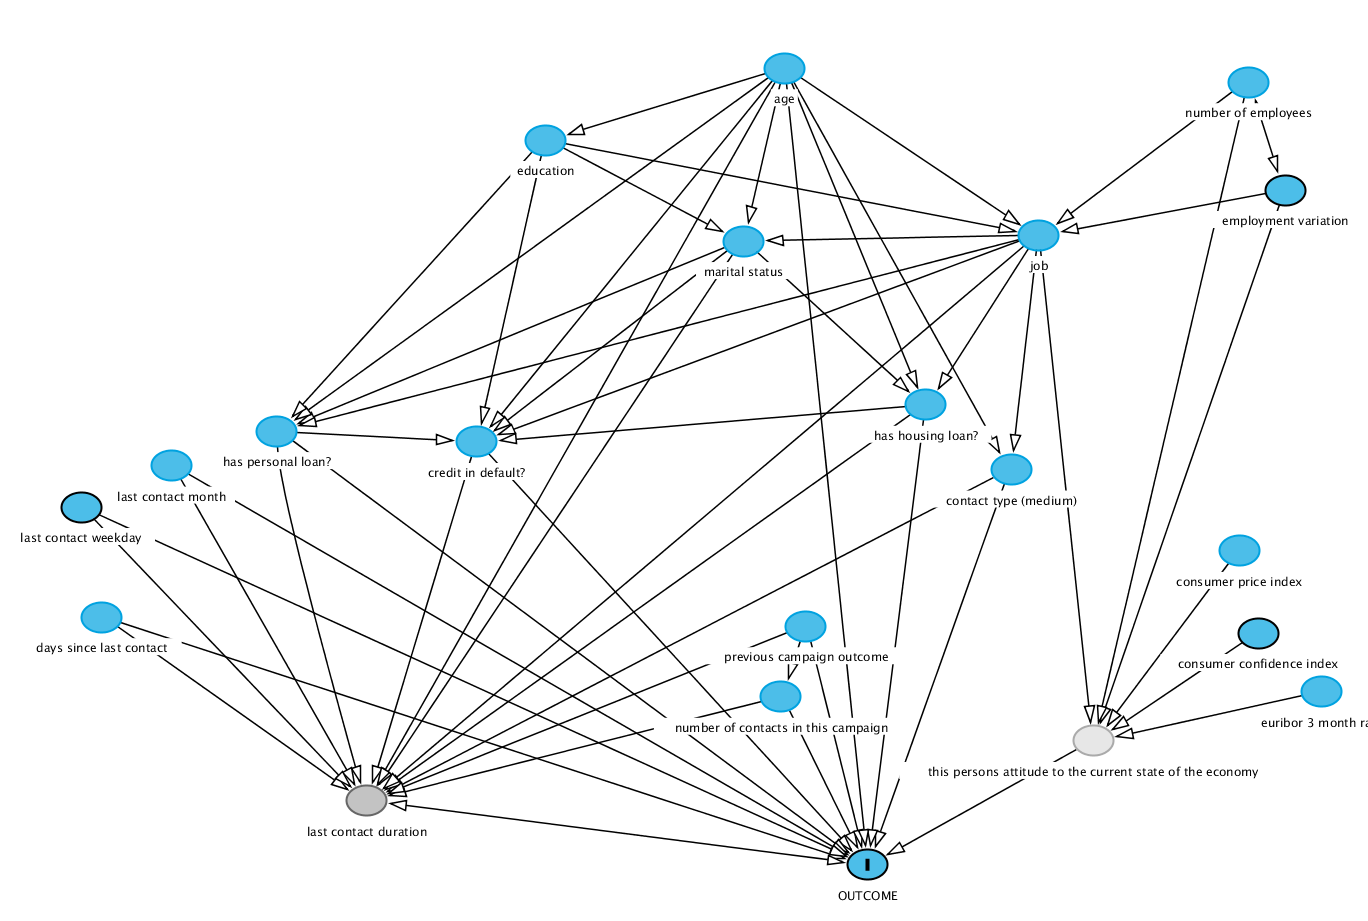
\includegraphics[width=0.9\textwidth]{images/initial_dag}
	\caption{Initial DAG as proposed in exposee.}
	\label{fig:initial_dag}
\end{figure}

\subsection{Derived Tests}
Conditional independencies were automatically derived using the \texttt{ImpliedLocalDependencies} function from the \texttt{dagitty} package in \texttt{R}.
{\tiny\begin{verbatim}
consumer confidence index _||_ consumer price index
consumer confidence index _||_ contact type (medium)
consumer confidence index _||_ credit in default?
consumer confidence index _||_ days since last contact
consumer confidence index _||_ employment variation
consumer confidence index _||_ euribor 3 month rate
consumer confidence index _||_ has housing loan?
consumer confidence index _||_ has personal loan?
consumer confidence index _||_ last contact duration
consumer confidence index _||_ last contact month
consumer confidence index _||_ last contact weekday
consumer confidence index _||_ marital status
consumer confidence index _||_ number of contacts in this campaign
consumer confidence index _||_ number of employees
consumer confidence index _||_ previous campaign outcome
consumer confidence index _||_ age
consumer confidence index _||_ education
consumer confidence index _||_ job
consumer price index _||_ contact type (medium)
consumer price index _||_ credit in default?
consumer price index _||_ days since last contact
consumer price index _||_ employment variation
consumer price index _||_ euribor 3 month rate
consumer price index _||_ has housing loan?
consumer price index _||_ has personal loan?
consumer price index _||_ last contact duration
consumer price index _||_ last contact month
consumer price index _||_ last contact weekday
consumer price index _||_ marital status
consumer price index _||_ number of contacts in this campaign
consumer price index _||_ number of employees
consumer price index _||_ previous campaign outcome
consumer price index _||_ age
consumer price index _||_ education
consumer price index _||_ job
contact type (medium) _||_ credit in default? | age, job
contact type (medium) _||_ days since last contact
contact type (medium) _||_ employment variation | age, job
contact type (medium) _||_ euribor 3 month rate
contact type (medium) _||_ has housing loan? | age, job
contact type (medium) _||_ has personal loan? | age, job
contact type (medium) _||_ last contact month
contact type (medium) _||_ last contact weekday
contact type (medium) _||_ marital status | age, job
contact type (medium) _||_ number of contacts in this campaign
contact type (medium) _||_ number of employees | age, job
contact type (medium) _||_ previous campaign outcome
contact type (medium) _||_ education | age, job
credit in default? _||_ days since last contact
credit in default? _||_ employment variation | age, education, job
credit in default? _||_ euribor 3 month rate
credit in default? _||_ last contact month
credit in default? _||_ last contact weekday
credit in default? _||_ number of contacts in this campaign
credit in default? _||_ number of employees | age, education, job
credit in default? _||_ previous campaign outcome
days since last contact _||_ employment variation
days since last contact _||_ euribor 3 month rate
days since last contact _||_ has housing loan?
days since last contact _||_ has personal loan?
days since last contact _||_ last contact month
days since last contact _||_ last contact weekday
days since last contact _||_ marital status
days since last contact _||_ number of contacts in this campaign
days since last contact _||_ number of employees
days since last contact _||_ previous campaign outcome
days since last contact _||_ age
days since last contact _||_ education
days since last contact _||_ job
employment variation _||_ euribor 3 month rate
employment variation _||_ has housing loan? | age, job, marital status
employment variation _||_ has housing loan? | age, education, job
employment variation _||_ has personal loan? | age, education, job
employment variation _||_ last contact duration | age, credit in default?, has housing loan?, has personal loan?, job, marital status
employment variation _||_ last contact duration | age, education, job
employment variation _||_ last contact month
employment variation _||_ last contact weekday
employment variation _||_ marital status | age, education, job
employment variation _||_ number of contacts in this campaign
employment variation _||_ previous campaign outcome
employment variation _||_ age
employment variation _||_ education
euribor 3 month rate _||_ has housing loan?
euribor 3 month rate _||_ has personal loan?
euribor 3 month rate _||_ last contact duration
euribor 3 month rate _||_ last contact month
euribor 3 month rate _||_ last contact weekday
euribor 3 month rate _||_ marital status
euribor 3 month rate _||_ number of contacts in this campaign
euribor 3 month rate _||_ number of employees
euribor 3 month rate _||_ previous campaign outcome
euribor 3 month rate _||_ age
euribor 3 month rate _||_ education
euribor 3 month rate _||_ job
has housing loan? _||_ has personal loan? | age, job, marital status
has housing loan? _||_ last contact month
has housing loan? _||_ last contact weekday
has housing loan? _||_ number of contacts in this campaign
has housing loan? _||_ number of employees | age, education, job
has housing loan? _||_ number of employees | age, job, marital status
has housing loan? _||_ previous campaign outcome
has housing loan? _||_ education | age, job, marital status
has personal loan? _||_ last contact month
has personal loan? _||_ last contact weekday
has personal loan? _||_ number of contacts in this campaign
has personal loan? _||_ number of employees | age, education, job
has personal loan? _||_ previous campaign outcome
last contact duration _||_ number of employees | age, education, job
last contact duration _||_ number of employees | age, credit in default?, has housing loan?, has personal loan?, job, marital status
last contact duration _||_ education | age, credit in default?, has housing loan?, has personal loan?, job, marital status
last contact month _||_ last contact weekday
last contact month _||_ marital status
last contact month _||_ number of contacts in this campaign
last contact month _||_ number of employees
last contact month _||_ previous campaign outcome
last contact month _||_ age
last contact month _||_ education
last contact month _||_ job
last contact weekday _||_ marital status
last contact weekday _||_ number of contacts in this campaign
last contact weekday _||_ number of employees
last contact weekday _||_ previous campaign outcome
last contact weekday _||_ age
last contact weekday _||_ education
last contact weekday _||_ job
marital status _||_ number of contacts in this campaign
marital status _||_ number of employees | age, education, job
marital status _||_ previous campaign outcome
marital status _||_ OUTCOME | age, credit in default?, employment variation, has housing loan?, has personal loan?, job, number of employees
marital status _||_ OUTCOME | age, credit in default?, education, has housing loan?, has personal loan?, job
number of contacts in this campaign _||_ number of employees
number of contacts in this campaign _||_ age
number of contacts in this campaign _||_ education
number of contacts in this campaign _||_ job
number of employees _||_ previous campaign outcome
number of employees _||_ age
number of employees _||_ education
previous campaign outcome _||_ age
previous campaign outcome _||_ education
previous campaign outcome _||_ job
OUTCOME _||_ education | age, credit in default?, employment variation, has housing loan?, has personal loan?, job, number of employees
\end{verbatim}}

\section{Approach}
Tests were performed automatically using the \texttt{localTests} function from the \texttt{dagitty} package.
However, we are dealing with attributes that can take on many different values, so we'll need to do some pre-processing first.
\begin{description}[align=right, leftmargin=2cm, labelwidth=3cm]
	\item[age] Discrete values between 18-85
	\item[nr.employed] continuous values
	\item[emp.var.rate] continuous values
	\item[cons.price.idx] continuous values
	\item[cons.conf.idx] continuous values
	\item[euribor3m] continuous values
\end{description}

\subsection{Binning}
Because \texttt{dagitty} interprets our data as nominal, it is necessary to bin our data to allow for meaningful analysis. For each of these attributes, we inspect the histogram of value frequencies + we apply domain knowledge to obtain acceptable bins.

%Voor elke subsectie nog wat tekst
\subsubsection{Age}
\begin{figure}[H]
	\centering
	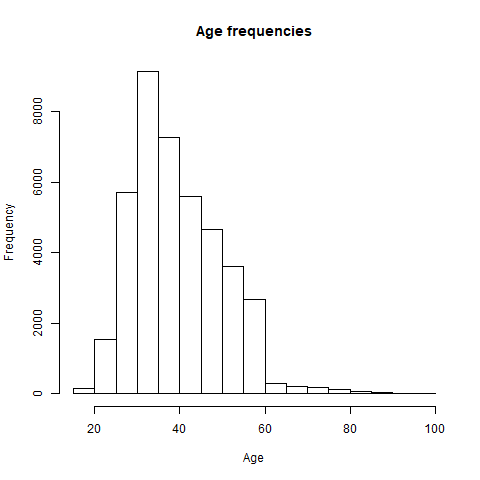
\includegraphics[width=0.4\textwidth]{images/age}
	\caption{Distribution of age.}
	\label{fig:age}
\end{figure}

\subsubsection{Quarterly average of number of employees}
\begin{figure}[H]
	\centering
	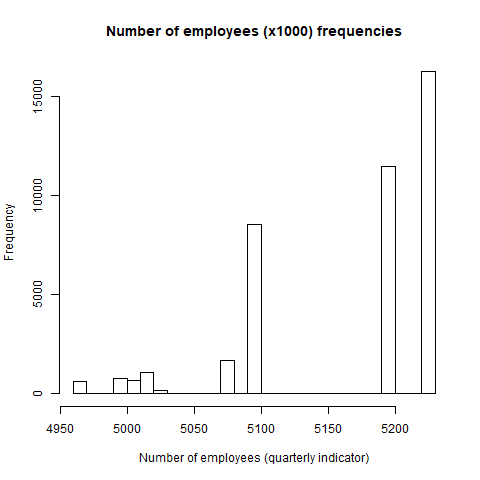
\includegraphics[width=0.4\textwidth]{images/nr_employed}
	\caption{Distribution of number of employees.}
	\label{fig:nr_employed}
\end{figure}

\subsubsection{Quarterly average of number of employees}
\begin{figure}[H]
	\centering
	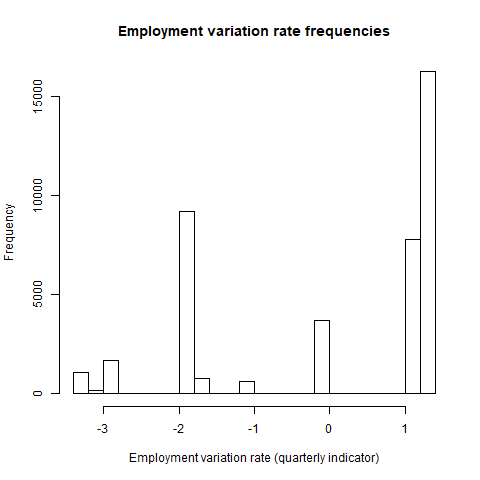
\includegraphics[width=0.4\textwidth]{images/emp_var_rate}
	\caption{Distribution of employment variation rate.}
	\label{fig:emp_var_rate}
\end{figure}

\subsubsection{Consumer price index}
\begin{figure}[H]
	\centering
	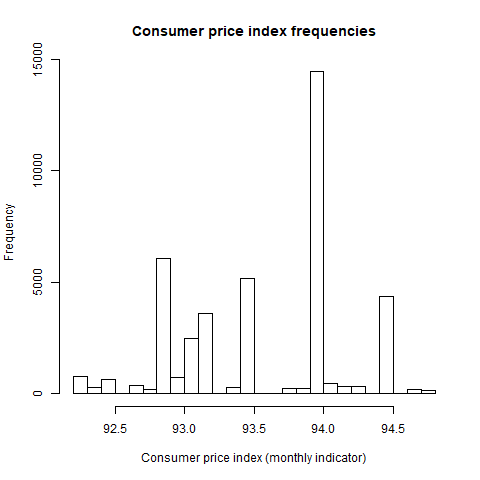
\includegraphics[width=0.4\textwidth]{images/consumer_price_index}
	\caption{Distribution of consumer price index.}
	\label{fig:cons_price_idx}
\end{figure}

\subsubsection{Consumer confidence index}
\begin{figure}[H]
	\centering
	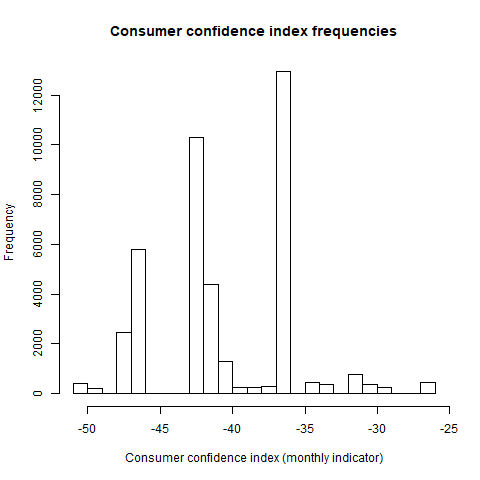
\includegraphics[width=0.4\textwidth]{images/consumer_confidence_index}
	\caption{Distribution of consumer confidence index.}
	\label{fig:cons_conf_idx}
\end{figure}

\subsubsection{Euribor 3 month rate}
\begin{figure}[H]
	\centering
	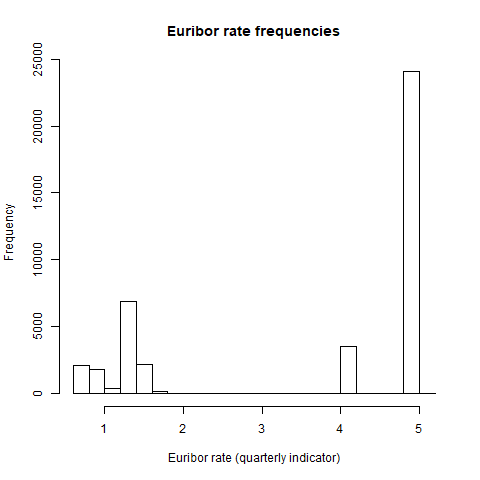
\includegraphics[width=0.4\textwidth]{images/euribor3m}
	\caption{Distribution of three month euribor rate.}
	\label{fig:euribor3m}
\end{figure}

\subsection{Testing method}
Prioriteit van tests: ja, in volgorde van oplopend aantal conditioning variables (0 tot geen limiet)
Runnen alles tegelijkertijd, maar voeren slechts 1 wijziging uit per keer, waarna we weer alles runnen.
Hoe quantificeerden we de testresultaten? RMSEA. (Uitleg?)

\section{Changes}
Verwerk hier het logboek + nog uit te voeren veranderingen.

\section{Revised DAG}
\end{document}